%章节
%\section{}, \subsection{}, \subsubsection{}, \paragraph{}, \subparagraph{}

%插入图片
%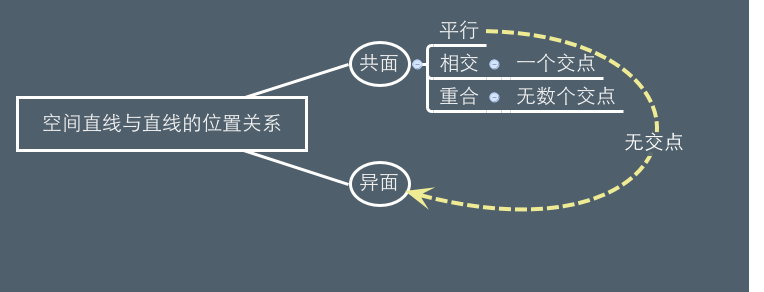
\includegraphics[height=100px]{/Users/shuyue/Desktop/1.png}

%无序列表
%\begin{itemize}
%\item
%\item
%\item
%\item 
%\end{itemize}

%有序列表
%\begin{enumerate}
%\item 
%\item
%\item
%\item
%\end{enumerate}

%嵌套列表
%\begin{itemize}
%\item
%\begin{enumerate}
%\item 
%\item 
%\item 
%\end{enumerate}
%\item
%\begin{enumerate}
%\item 
%\item 
%\item 
%\end{enumerate}
%\end{itemize}

%分栏
%\begin{multicols}{2}
%1\columnbreak \\ 2
%\end{multicols}

%标号
%\textcircled{1}

\documentclass[a4,12pt]{article}
\RequirePackage{CJKutf8,hyperref,mathtools,amssymb,geometry,enumerate,multicol,graphicx,dcolumn}

\begin{document}
\begin{CJK}{UTF8}{gkai}

\title{小数的减法}
\date{}
\author{张舒悦}
\maketitle

\section{教学目标}
\begin{enumerate}
\item 理解和掌握小数减法的计算方法, 能正确地计算小数减法.
\item 熟练地口算有效数字为两位的小数减法.
\item 初步掌握小数的加减混合运算.
\end{enumerate}

\section{教学重点}
\begin{enumerate}
\item 体会小数减法的算理.
\item 掌握小数减法的计算方法.
\end{enumerate}

\section{教学难点}
\begin{enumerate}
\item 被减数是整数或小数位数比减数小数位数少的小数减法.
\end{enumerate}

\section{教学过程}

回顾小数的加法运算关键点: 数位对齐$\Leftrightarrow$小数点对齐.\\
减法是加法的逆运算; 减法和加法是同级运算.\\
引入情景, 由总成绩和后掷成绩计算前掷成绩.
$$11.4-6.17=?$$

\subsection{整数的减法}
$$131-12=?$$
小数点对齐, 列竖式演算.\\
借位是因为对应数位上的数字不够被减.

\subsection{小数的减法}
列竖式演算时, 小数点要对齐.\\
小数减法法则:
\begin{enumerate}
\item 小数点对齐.
\item 按整数减法法则进行计算.
\item 可去除得数小数部分末尾的"0".
\end{enumerate}
演示完成$11.4-6.17.$\\
\vspace{7mm}\\
\begin{tabular}{cD{.}{.}{2}}
&11.4\\
- &6.17\\
\hline
& 5.23
\end{tabular}
\vspace{7mm}\\
引导和解释添0和借位.

\subsection{竖式练习}
列竖式计算$11-4.9 .$\\
\vspace{7mm}\\
\begin{tabular}{cD{.}{.}{1}}
&11\\
- &4.9\\
\hline
& 6.1
\end{tabular}

\subsection{书后练习}
a 独立完成.
b 组织同学讨论.

\subsection{加减混合运算}
计算$$2.3-0.53+2.1=3.87 .$$
计算$$7.3-(2.1-0.92)=6.12 .$$

\subsection{书后练习}
d e 讲解备选.
c 完成后, 一个个批阅.

\section{小结}
\begin{enumerate}
\item 小数的减法运算法则.
\item 小数加减法的运算法则异同.
\end{enumerate}

\section{作业}
\begin{enumerate}
\item 订正练习册和一课一练.
\item 练习册 P28.
\item 一课一练 P55-56.
\end{enumerate}

\end{CJK}
\end{document}